\documentclass{../notatki}

\title{Uczenie Głębokie}

\begin{document}

\section{Problem}

Chcemy na podstawie zawczasu znanego zbioru danych $X \in
\mathbb{R}^{n \times d}$, i odpowiadających
nim etykiet $y$, przewidywać etykiety $\hat{y}(x)$ dla nowych punktów
$x \notin X$.

Standardowo, w problemach klasyfikacji, dzielimy dzielimy dane na zbiór
treningowy, walidacyjny oraz testowy. Trenujemy na treningowym, dobieramy
hiperparametry na walidacyjnym, a potem ewaluujemy na testowym. Bardziej
niezawodnym mechanizmem ewaluacji jest walidacja krzyżowa
(cross-validation), gdzie w kolejnych iteracjach wybieramy różne
podzbiory danych jako zbiór treningowy i walidacyjny.

\section{Nearest Neighbor}

\begin{enumerate}
  \item Zapamiętujemy wzystkie $X$ i $y$
  \item Przewidujemy klasę $\hat{y}(x)$ dla $x \notin X$, taką, że dla danej
    metryki odległości $d$:
    $$
    \hat{y}(x) = \arg\min_{y_i \in Y} d(x, X_i)
    $$
\end{enumerate}

Aby przeciwdziałać szumowi w danych, można brać próbkę $\{y_1, y_2,
\dots, y_k\}$, $k$ najbliższych sąsiadów, a potem brać średnią z tych klas.

Można używać różnych $d$, np:
\begin{itemize}
  \item $d(a, b) = l_1(a, b) = \sum_{i=1}^n |a_i - b_i|$
  \item $d(a, b) = l_2(a, b) = \sqrt{\sum_{i=1}^n (a_i - b_i)^2}$
\end{itemize}

Problemem jest złożoność obliczeniowa, naiwna wersja algorytmu musi pamiętać
wszystkie $X$ i $y$ w pamięci, a potem dla każdego nowego punktu $x$ musi
przeszukiwać wszystkie $X$.

\section{Regresja Liniowa}

Modele nearest neighbor dynamicznie określają granicę między punktami,
natomiast regresja liniowa stara się znaleźć prostą, która najlepiej
rozdziela etykiety $y$ na podstawie $X$.

Dla każdej klasy $y_i$, definiujemy wektor wag $W_i \in
\mathbb{R}^d$, i bias $b_i \in \mathbb{R}$. Potem, określamy funkcję
\texttt{score}:
$$
f_i(x, W, b) = W_i \cdot x + b_i \quad \hat{y}(x) = \arg\max_{y_i} f_i(x, W, b)
$$

Problemem dla klasyfikatorów tego typu, oczywiście, jest kształt
danych. W zależności, od przyjętej przestrzeni $\mathbb{R}^d$, dane
mogą być liniowo separowalne, ale w ogólności nie są.

\section{Loss i regularyzacja}

Aby określić jakość predykcji, dla danej funkcji $f_i(x, W, b)$,
definiujemy funkcję straty (loss):
$$
L(W, b) = \frac{1}{n} \sum_{i=1}^n L_i(W, b)
$$
czyli średnia straty dla wszystkich próbek.

Aby zapobiec overfittingu, stosuje się regularyzację. W regularyzacji, dodajemy
do $L$, karę, która jest proporcjonalna do \textit{skomplikowania} modelu. W
ten sposób model jest nagradzany za generalizowanie.
$$
L(W, b) = \frac{1}{n} \sum_{i=1}^n L_i(W, b) + \lambda R(W)
$$
Jest wiele potencjalnych mechanizmów regularyzacji:
\begin{itemize}
  \item $R_2(W) = \sum_k \sum_l W_{k,l}^2$ - L2
  \item $R_1(W) = \sum_k \sum_l |W_{k,l}|$ - L1
  \item $R_{1 + 2}(W) = \sum_k \sum_l \beta W_{k,l}^2 + |W_{k,l}|$ -
    L1 + L2 (Elastic net)
  \item Dropout
  \item Batch norm
  \item \dots
\end{itemize}

\begin{examplebox}
  Wyobraźmy sobie, dwie różne macierze $W_1$ i $W_2$, do modelu liniowego.
  Mają one rozróżnić $x_0$ i $x_1$.
  $$
  x_0 =
  \begin{bmatrix}
    1 \\
    1 \\
    1 \\
    1
  \end{bmatrix} \quad x_1 =
  \begin{bmatrix}
    1 \\
    0 \\
    0 \\
    0
  \end{bmatrix}
  \quad
  W_0^T =
  \begin{bmatrix}
    0 \\
    0 \\
    0 \\
    1
  \end{bmatrix} \quad W_1^T =
  \frac{1}{3}
  \begin{bmatrix}
    0 \\
    1 \\
    1 \\
    1
  \end{bmatrix}
  $$
  $$
  \quad W_0 x_0 = 1 = W_1 x_0\quad \neq \quad W_0 x_1 = 0 = W_1 x_1
  $$
  Lecz, regularyzacja L2 $R_2(W)$, potrafi daje inne wyniki dla $W_0$ i $W_1$:
  $$
  R_2(W_0) = 1 \quad \neq \quad R_2(W_1) = 3 \cdot \frac{1}{9} = \frac{1}{3}
  $$
  Więc, przy zastosowaniu regularyzacji L2, $W_0$ i $W_1$ nie są równoważne,
  i podczas optymalizacji, algorytm będzie preferował $W_1$, ponieważ
  ma mniejszą wartość regularyzacji.
\end{examplebox}

\subsection{SVM}

Wieloklasowy SVM $L_i$, dla próbki $(x_i, y_i)$ ma postać:
$$
L_i(W, b) = \sum_{j \neq i} \max(0, f_j(x_i, W, b) - f_i(x_i, W, b) + 1)
$$
Intuicyjnie, jest to ograniczona przez $0$ od dołu suma różnic,
między \texttt{score} każdej innej klasy, a docelowej klasy.

\subsection{Softmax loss}

$$
L_i(W, b) = -\log P(y = i | x) = -\log \left(\frac{e^{f_i(x, W,
b)}}{\sum_j e^{f_j(x, W, b)}}\right)
$$

\section{Optymalizacja}

$$
W = \arg\min_w L(w)
$$

\subsection{Gradient Descent}

Dla $t$-tego kroku optymalizacji:
$$
W_{t} = W_{t-1} - \alpha \nabla L(W_{t-1})
$$
realizujemy ten krok, aż nie napotkamy na warunek stopu ($\nabla L \approx 0$),
lub osiągniemy maksymalną liczbę iteracji. Oczywiście, trzeba jakoś określić
$W_0$, czyli punkt startowy optymalizacji, tutaj zazwyczaj jest to
losowa wartość. Kluczowym, z kolei, jest $\alpha$, czyli \textit{learning rate}.
Tutaj jest to zazwyczaj \textit{problem-specific}.

\subsubsection{Batch GD}

W Batch GD, aby zapobiec obliczaniu całkowitej funkcji straty, co
jest problematyczne dla dużych zbiorów danych, obliczamy funkcję
straty na całym zbiorze danych w każdej iteracji.

\subsubsection{Stochastic GD}

W Stochastic GD, na odwrót, obliczamy funkcję straty tylko dla jednej
losowo wybranej próbki w każdej iteracji.

\subsection{Momentum}

Jeśli, założymy jakiś poziom racjonalności problemu optymalizacji, to przydatnym
może być zastosowanie \textit{momentum}. Momentum $v$ jest zdefiniowane jak
pęd fizyczny;
$$
v_{t} = \rho v_{t-1} + \nabla L(W_{t-1})
$$
W interpretacji fizycznej, $v$ jest prędkością, a $\rho$
współczynnikiem tłumienia - tarciem.

Dla $t$-tego kroku optymalizacji:
$$
W_{t} = W_{t-1} - \alpha v_{t}
$$

\subsection{AdaGrad}

Alternatywnym mechanizmem jest zachowywanie historycznej sumy
kwadratów gradientów i używanie jej do skalowania współczynnika
uczenia $\alpha$.
$$
\nabla^2_t = \sum_{i=1}^{t} \nabla L(W_i)^2
$$
$$
W_t = W_{t - 1} - \frac{\alpha}{\sqrt{\nabla^2_t} + \epsilon} \cdot
\nabla L(W_{t-1})
$$

\subsection{RMSProp}

Jest to modyfikacja AdaGrad, która wprowadza \textit{decay rate} w
obliczaniu $\nabla^2_t$.
$$
\nabla^2_t = \sum_{i=1}^{t} \rho \nabla^2_{i} + (1 - \rho)
\cdot \nabla L(W_i)^2
$$

\subsection{Adam}

Adam to połączenie \textit{momentum} i \textit{RMSProp}. Pamięta on dwa pierwsze
momenty ruchu: $v$ - prędkość, $m$ - moment. Aby zapobiec problemu z
$v_0 = 0, m_0 = 0$, który może wystąpić w pierwszej iteracji, stosuje
się \textit{bias correction} $v'_t$ i $m'_t$.
$$
v_t = \beta_1 m_{t-1} + (1 - \beta_1) \cdot \nabla L(W_{t-1}) \quad
v'_t = \frac{v_t}{1 - \beta_1^t}
$$
$$
m_t = \beta_2 m_{t-1} + (1 - \beta_2) \cdot \nabla L(W_{t-1})^2 \quad
m'_t = \frac{m_t}{1 - \beta_2^t}
$$
$$
W_t = W_{t-1} - \frac{\alpha v'_t}{\sqrt{m'_t} + \epsilon}
$$

\section{Sieci neuronowe}

Zamiast stosować pojedyncze modele liniowe, stosujemy je w $k$ warstwach,
gdzie każda warstwa się składa z $j$ neuronów. Każdy neuron w warstwie
$l$ ma wejście z warstwy $l-1$ i wyjście do warstwy $l+1$.

Dla $3$-warstwowej sieci neuronowej, o funkcji aktywacji $\sigma$:
$$
f(x) = W_3 \sigma(W_2 \sigma(W_1 \cdot x))
$$

\subsection{Funkcje aktywacji}

Można stosować wielu różnych funkcji aktywacji:
\begin{itemize}
  \item \textit{ReLU}: $f(x) = \max(0, x)$
  \item \textit{Sigmoid}: $f(x) = \frac{1}{1 + e^{-x}}$
  \item \textit{Tanh}: $f(x) = \tanh(x)$
  \item \textit{Leaky ReLU}: $f(x) = \max(0.01x, x)$
  \item \dots
\end{itemize}
Pozwalają one, na transformacje danych wejściowych, co ma pozwolić na liniową
separowalność danych.

\subsection{Konwolucja}

Warstwy konwolucyjne są używane do ekstrakcji cech z danych wejściowych,
takich jak obrazy. Dana warstwa konwolucyjna, ma do czynienia z pewną warstwą
danych wejściowych, oraz filtrem, którego się uczy, aby wyodrębnić cechy z
danych wejściowych. Hiperparametrem warstwy konwolucyjnej jest rozmiar filtra,
oraz stride, który określa, co ile pikseli przesuwać filtr po obrazie.

\begin{examplebox}
  Dla filtra $3\times3$, i stride $1$:
  $$
  \begin{bmatrix}
    \textcolor{red}{3} & \textcolor{red}{0} & \textcolor{red}{1} & 2 \\
    \textcolor{red}{1} & \textcolor{red}{5} & \textcolor{red}{8} & 9 \\
    \textcolor{red}{2} & \textcolor{red}{7} & \textcolor{red}{2} & 5 \\
    0 & 1 & 3 & 1
  \end{bmatrix}
  *
  \begin{bmatrix}
    1 & 0 & -1 \\
    1 & 0 & -1 \\
    1 & 0 & -1
  \end{bmatrix}
  =
  \begin{bmatrix}
    \textcolor{red}{-5} & -4 \\
    -10 & -2
  \end{bmatrix}
  $$
  $$
  \textcolor{red}{3 + 1 + 2 - 1 - 8 - 2 = -5}
  $$
\end{examplebox}

\subsection{Pooling}

Warstwy pooling są używane do zmniejszenia rozmiaru danych wejściowych,
takich jak obrazy. Działają one na danych wyjściowych warstwy konwolucyjnej,
redukując ich rozmiar poprzez wybieranie maksymalnych wartości w
podprzedziałach. Dla danego \textit{stride}, \textit{kernel size} i danych
wejściowych, warstwa pooling nakłada pewną prostą operację na danych.

\begin{examplebox}
  Dla \texttt{MaxPool} $2\times2$ i stride $2$:
  $$
  \begin{bmatrix}
    \textcolor{red}{3} & \textcolor{red}{0} & 1 & 2 \\
    \textcolor{red}{1} & \textcolor{red}{5} & 8 & 9 \\
    2 & 7 & 2 & 5 \\
    0 & 1 & 3 & 1
  \end{bmatrix} \Rightarrow
  \begin{bmatrix}
    \textcolor{red}{5} & 9\\
    7 & 5
  \end{bmatrix}
  $$
\end{examplebox}

\subsection{Residual Networks}

Im głębsze sieci są, tym większy mają problem z propagacją gradientu.
Na gradient, największy wpływ ma ostatnia warstwa. Im głębiej, tym mniejszy
jest wpływ na wyjście, aż w końcu, po $\approx 10$ warstwach, pierwsza
warstwa ma wpływ mniejszy niż dokładność \texttt{float32}.

Rozwiązaniem tego problemu jest użycie \textit{residual connections}, które
pozwalają propagować gradient przez głębokie sieci, nawet gdy gradient
jest bardzo mały w ostatniej warstwie.

Dla warstwy $F_i(x)$, zdefiniujmy:
$$
F_i(x) = F_{i-1}(x) + x
$$
W pewnym sensie zatem, sieć się uczy odwzorowywać innej funkcji, ale
w klasyfikacji wewnętrzny stan numeryczny sieci nas nie interesuje.

\section{Wizja komputerowa}

Dotychczas rozważaliśmy tylko klasyfikację. Co jeśli nas interesuje konkretnie
pozycja obiektu na obrazie? Jest to problem regresji, a nie klasyfikacji.
Tutaj, musimy traktować jako wyjście kilka mniejszych zmiennych regresyjnych,
każda odpowiadająca za jedną współrzędną: $p = (x, y, w, h)$.

Powszechnym, w abstrakcyjnym kontekście detekcji obrazów, jest pre-trenowany
transformer, który się składa tylko z warstw konwolucyjnych, który potem
jest łączony z konkretną architekturą detekcji, w zależności od zadania.

\subsection{Region-based}

Aby zrealizować region-based detekcję, czyli detekcje konkretnej pozycji
na obrazie, często stosowana jest region-based detekcja. Naiwną realizacją
tej ideii, jest aplikowanie modelu klasyfikacji, dla wszystkich pod-obrazów
w obrazie, a następnie wybór pod-obrazu, dla którego model zwrócił najwyższy
wynik. Bardziej zaawansowane podejścia zazwyczaj stosują heurystyczny wybór
regionów, które mogą nas interesować.

\subsection{IoU}

Aby porównać wynik modelu $\hat{p}$ z rzeczywistą pozycją obiektu $p$,
często stouje się IoU (Intersection over Union), lub index Jaccarda.
$$
IoU(p, \hat{p}) = \frac{p \cap \hat{p}}{p \cup \hat{p}}
$$

\subsection{NMS}

Aby wyeliminować nadmiarowe detekcje, stosuje się NMS (Non-Maximum Suppression).
\begin{enumerate}
  \item Wybieramy $\hat{p}' = \arg\max_{\hat{p}} IoU(p, \hat{p})$
  \item Eliminujemy wszystkie $\hat{p}$, dla których $IoU(\hat{p}',
    \hat{p}) > \theta$
  \item Wracamy do kroku 1
\end{enumerate}
Intuicyjnie, dla każdego optymalnego $\hat{p}'$, eliminujemy wszystkie zbyt
podobne, lecz gorsze, predykcje, aż zostają tylko optymalne wyspy, zbyt różne
aby odrzucić.

\subsection{mAP}

mAP (mean Average Precision) jest miarą oceny modelu klasyfikacji, która
względem IoU (Intersection over Union) określa, jak dobrze model
odpowiada na dane testowe.

\begin{enumerate}
  \item Stosujemy NMS
  \item Dla każdej kategorii, obliczamy Average Precision (AP),
    zdefiniowane jako powierzchnia pod krzywą Precision-Recall (PR)
    dla tej kategorii
    \begin{enumerate}
      \item Dla każdego przewidzianego punktu $\hat{p}$
      \item Jeśli pokrywa się z jakimś rzeczywistym punktem $p$ z
        $IoU(\hat{p}, p) > \theta$, oznacz go jako pozytywny
      \item W p.p. oznacz go jako negatywny
      \item Dodaj punkt do PR curve, z aktualnym stanem precyzji (\%
        $\hat{p}$ pozytywnych) i czułości (\% $p$ z przyporządkowanym $\hat{p}$)
    \end{enumerate}
  \item AP dla kategorii to powierzchnia pod krzywą PR dla tej kategorii
  \item mAP to średnia AP dla wszystkich kategorii
\end{enumerate}

Intuicyjnie, dla danej kategorii, szukamy, czy każda predykcja ma match
w ground truth, mierzymy ile predykcji ma, oraz jakość predykcji. Nasz
performance w czasie mierzymy, poprzez powierzchnię pod krzywą PR, i
to nam daje AP. Potem uśredniamy AP dla
wszystkich kategorii, aby uzyskać mAP.

\begin{examplebox}

  Uruchamiamy klasyfikator na różnych regionach, to nam zwraca sporo predykcji.
  Eliminujemy je przy pomocy NMS.
  Mamy pięć predykcji $\hat{p}_i$ i trzy rzeczywiste punkty $p_j$.

  Zaczynając od punktów z największą wewnętrzną pewnością, szukamy
  odpowiadającego mu punktu $p$. Jest taki, to możemy go usunąć. Aktualnie mamy
  prezycję $\frac{1}{1}$, oraz czułość $\frac{1}{3}$. Dodajemy punkt do krzywej
  i kotynuujemy.

  \dots

  Na koniec zostaje nam ciąg punktów krzywej PR: $\left(1,
  \frac{1}{3}\right), \left(\frac{2}{2}, \frac{2}{3}\right),
  \left(\frac{2}{3}, \frac{2}{3}\right), \left(\frac{2}{4},
  \frac{2}{3}\right), \left(\frac{3}{5}, \frac{3}{3}\right)$.

  \begin{center}
    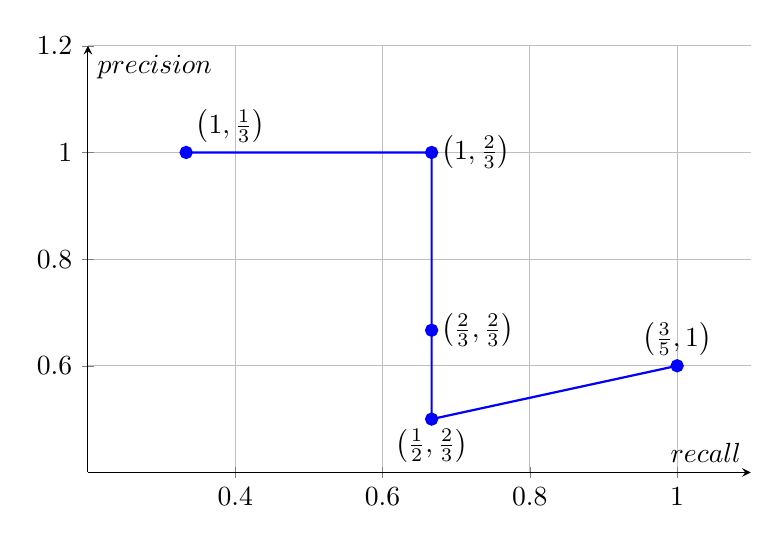
\begin{tikzpicture}
      \begin{axis}[
          width=10cm,
          height=7cm,
          axis lines=middle,
          xlabel={$recall$},
          ylabel={$precision$},
          xmin=0.2, xmax=1.1,
          ymin=0.4, ymax=1.2,
          grid=both,
        ]
        % Polyline through the points
        \addplot[
          blue,
          thick,
          mark=*,
        ] coordinates {
          (1/3,1)
          (2/3,1)
          (2/3,2/3)
          (2/3,1/2)
          (1,3/5)
        };

        % Optional labels
        \node[above right] at (axis cs:1/3,1) {$\left(1,\frac13\right)$};
        \node[right]       at (axis cs:2/3,1) {$\left(1,\frac23\right)$};
        \node[right]       at (axis cs:2/3,2/3)
        {$\left(\frac23,\frac23\right)$};
        \node[below]       at (axis cs:2/3,1/2)
        {$\left(\frac12,\frac23\right)$};
        \node[above]       at (axis cs:1,3/5) {$\left(\frac35,1\right)$};
      \end{axis}
    \end{tikzpicture}
  \end{center}
  Powierzchnia pod tą krzywą to nasz AP.

\end{examplebox}

\subsection{Fast R-CNN}

Zamiast odpalać nasz klasyfikator, tyle razy, ile mamy regionów, to odpalamy
nasz \textit{backbone} feature extractor, raz. Na tej przestrzeni potem
odnajdujemy regiony i robimy klasyfikację. W ten sposób, część
obliczeń jest wykonywana tylko raz.

Tutaj, jedynym problemem jest cropping czynników. Dostaliśmy z naszej
heurystyki regionów jakieś croppy, a potrzebujemy je przenieść na
przestrzeń czynników, lecz nasza wyekstraktowana
przestrzeń cech nie rzutuje się 1:1 na obrazek wejściowy.

\subsubsection{Rol Pool}

\begin{enumerate}
  \item Rzutujemy obrazek na przestrzeń cech
  \item Niedokładne rzutowanie rozwiązujemy przez zaokrąglenie; "\textit{snap}"
  \item Dzielimy rzutowanie na grid $2\times 2$ regionów
  \item W ramach regionów robimy \textit{max pooling}
\end{enumerate}

Max pooling na koniec zapewnia, że niezależnie od rozmiaru regionu, zawsze mamy
ten sam rozmiar wyjściowy. Problemem, jest samo zaokrąglanie, które dodaje
niestabilność do uczenia i predykcji, szczególnie w dziwnych miejscach.

\subsubsection{Rol Align}

Jest to bardzo podobna metoda to \textit{Rol Pool}, lecz, zamiast zaokrąglenia,
wykorzystuje interpolację. Jak dostajemy punkt regionu między czynnikami
przestrzeni czynników, definujemy nowy czynnik, jako kombinację
liniową czynników przestrzeni, w taki sposób, że punkt regionu jest w
środku nowego czynnika.

Intuicyjnie, zamiast zaokrąglenia, interpolujemy i uśredniamy różnice między
regionami na obrazku, a przestrzenią czynników.

\subsection{RPN}

Zamiast heurystycznie szukać regionów, do konkretnego problemu, możemy
nauczyć sień neuronową, aby to robiła za nas.

\section{Segmentacja Semantyczna}

W semantycznej segmentacji, każdemu pikselowi chcemy przyporządkować pewną
klasę semantyczną w obrazku.
Naiwnym rozwiązaniem jest, po raz kolejny, przesuwanie okienka kontekstowego
i aplikowanie modelu klasyfikacyjnego na każdym pikselu.

\subsection{U-net}

Bardziej kompleksowym rozwiązaniem jest pełna konwolucyjna sieć neuronowa (CNN),
która jest trenowana na całym obrazie i każdemu pikselowi
przyporządkowuje klasę semantyczną. Problemem, jest ograniczone
\textit{receptive field} każdej warstwy konwolucyjnej, oraz koszta związane z
tym podejściem.

Tutaj, standardowo, stosuje się kombinacje downsamplingu i upsamplingu,
aby zwiększyć \textit{receptive field} każdej warstwy konwolucyjnej.
Downsampling to prosta sprawa, pooling jest rodzajem downsamplingu, który
zredukuje rozmiar obrazu poprzez agregację pikseli w oknach.

\subsection{Upsampling}

Jest wiele sposobów, na który można robić upsampling:
\begin{itemize}
  \item Bed of Nails - nadaj nowym komórkom wartość $0$
  \item Nearest Neighbor - nadaj nowym komórkom wartość najbliższego sąsiada
  \item Bilinear Interpolation - użyj dwóch najbliższych sąsiadów w
    obydwu wymiarach i skonstruuj interpolację liniową
  \item Bicubic Interpolation - użyj trzech najbliższych sąsiadów w
    obydwu wymiarach i skonstruuj interpolację kubiczną
  \item Max-Unpooling - przy downsamplingu zapamiętujemy pozycję największych
    wartości w każdym oknie, a przy upsamplingu przywracamy w te pozycje
    wartości
\end{itemize}

\begin{examplebox}
  $$
  \begin{bmatrix}
    1 & 2 & 6 & 3 \\
    3 & \textcolor{red}{5} & 2 & 1 \\
    1 & 2 & 2 & 1 \\
    7 & 3 & 4 & 8
  \end{bmatrix} \Rightarrow
  \begin{bmatrix}
    \textcolor{red}{5} & 6 \\
    7 & 8
  \end{bmatrix}
  \Rightarrow \dots \Rightarrow
  \begin{bmatrix}
    \textcolor{red}{1} & 2 \\
    3 & 4
  \end{bmatrix}
  \Rightarrow
  \begin{bmatrix}
    0 & 0 & 2 & 0 \\
    0 & \textcolor{red}{1} & 0 & 0 \\
    0 & 0 & 0 & 0 \\
    3 & 0 & 0 & 4
  \end{bmatrix}
  $$
\end{examplebox}

\section{RNN}

Rekurencyjne sieci neuronowe (RNN) są sieciami neuronowymi, które przetwarzają
dane sekwencyjne, gdzie każdy element sekwencji jest przetwarzany w kontekście
poprzednich elementów. Kluczowym konceptem, jest tak zwany
\textit{hidden state}.
$$
h_t = f_W(h_{t-1}, x_t) \quad y_t = g(h_t)
$$
W zależności od problemu, możemy mieć do czynienia z tylko jednym
wejściem zamiast $t$ wejść, oraz jednym wyjściem zamiast $t$ wyjść. To wszystko
zależy od problemu, który chcemy rozwiązać.

\begin{figure}
  \centering
  \resizebox{0.8\textwidth}{!}{%
    \begin{tikzpicture}[
        >=Stealth,
        every node/.style={font=\Large},
        hidden/.style={
          draw,
          fill=green!20,
          minimum width=1.6cm,
          minimum height=2.2cm
        },
        output/.style={
          draw,
          fill=blue!20,
          minimum width=1.6cm,
          minimum height=2.2cm
        },
        func/.style={
          draw,
          fill=gray!15,
          minimum width=1.8cm,
          minimum height=1.8cm
        },
        input/.style={
          draw,
          fill=red!20,
          minimum width=1.3cm,
          minimum height=2.2cm
        },
        weight/.style={
          draw,
          fill=orange!20,
          minimum width=1.6cm,
          minimum height=2cm
        },
        loss/.style={
          draw,
          fill=violet!20,
          minimum width=1.3cm,
          minimum height=1.0cm
        },
        total/.style={
          draw,
          fill=violet!20,
          minimum width=1.7cm,
          minimum height=1.5cm
        }
      ]

      %--------------------------------------------------
      % Main RNN chain
      %--------------------------------------------------

      \node[hidden] (h0) {$h_0$};

      \node[func, right=1.2cm of h0] (f1) {$\mathrm{f}_{W}$};
      \node[hidden, right=1.2cm of f1] (h1) {$h_1$};

      \node[func, right=1.2cm of h1] (f2) {$\mathrm{f}_{W}$};
      \node[hidden, right=1.2cm of f2] (h2) {$h_2$};

      \node[func, right=1.2cm of h2] (f3) {$\mathrm{f}_{W}$};
      \node[hidden, right=1.2cm of f3] (h3) {$h_3$};

      \node[hidden, right=5.0cm of h3] (hT) {$h_T$};

      %--------------------------------------------------
      % Outputs
      %--------------------------------------------------

      \node[output, above=1.1cm of h1] (y1) {$y_1$};
      \node[output, above=1.1cm of h2] (y2) {$y_2$};
      \node[output, above=1.1cm of h3] (y3) {$y_3$};
      \node[output, above=1.1cm of hT] (yT) {$y_T$};

      %--------------------------------------------------
      % Inputs
      %--------------------------------------------------

      \node[input, below=1.2cm of f1] (x1) {$x_1$};
      \node[input, below=1.2cm of f2] (x2) {$x_2$};
      \node[input, below=1.2cm of f3] (x3) {$x_3$};

      %--------------------------------------------------
      % Shared weights
      %--------------------------------------------------

      \node[weight, below left=1.8cm and 1.7cm of f1] (W) {$W$};

      %--------------------------------------------------
      % Losses
      %--------------------------------------------------

      \node[loss, right=1.0cm of y1] (L1) {$L_1$};
      \node[loss, right=1.0cm of y2] (L2) {$L_2$};
      \node[loss, right=1.0cm of y3] (L3) {$L_3$};
      \node[loss, right=1.0cm of yT] (LT) {$L_T$};

      \node[total, above right=1.8cm and 0.8cm of LT] (L) {$L$};

      %--------------------------------------------------
      % Forward recurrence
      %--------------------------------------------------

      \draw[->] (h0) -- (f1);
      \draw[->] (f1) -- (h1);

      \draw[->] (h1) -- (f2);
      \draw[->] (f2) -- (h2);

      \draw[->] (h2) -- (f3);
      \draw[->] (f3) -- (h3);

      \draw[->] (h3) -- ++(1.3,0);
      \draw[->] ($(hT.west)+(-1.1,0)$) -- (hT);

      %--------------------------------------------------
      % Outputs
      %--------------------------------------------------

      \draw[->] (h1) -- (y1);
      \draw[->] (h2) -- (y2);
      \draw[->] (h3) -- (y3);
      \draw[->] (hT) -- (yT);

      %--------------------------------------------------
      % Inputs to cells
      %--------------------------------------------------

      \draw[->] (x1) -- (f1);
      \draw[->] (x2) -- (f2);
      \draw[->] (x3) -- (f3);

      %--------------------------------------------------
      % Shared parameter arrows
      %--------------------------------------------------

      \draw[->]
      (W) to[out=60,in=-140]
      (f1.south west);

      \draw[->]
      (W.east) .. controls +(2,-0.4) and +(-1.0,-1.4) ..
      (f2.south);

      \draw[->]
      (W.east) .. controls +(4,-0.8) and +(-1.0,-1.4) ..
      (f3.south);

      %--------------------------------------------------
      % Per-step losses
      %--------------------------------------------------

      \draw[->] (y1) -- (L1);
      \draw[->] (y2) -- (L2);
      \draw[->] (y3) -- (L3);
      \draw[->] (yT) -- (LT);

      %--------------------------------------------------
      % Loss aggregation
      %--------------------------------------------------

      \draw[->]
      (L1.north)
      .. controls +(0,1.0) and +(-3.0,-0.3) ..
      (L.west);

      \draw[->]
      (L2.north)
      .. controls +(0,0.9) and +(-2.0,-0.2) ..
      (L.west);

      \draw[->]
      (L3.north)
      .. controls +(0,0.8) and +(-1.0,-0.3) ..
      (L.west);

      \draw[->]
      (LT.north)
      .. controls +(0,0.7) and +(0,-0.8) ..
      (L.south);

      %--------------------------------------------------
      % Ellipsis
      %--------------------------------------------------

      \node[scale=2.5] at ($(h3)!0.5!(hT)$) {$\cdots$};

    \end{tikzpicture}
  }
  \caption{Ilustracja architektury RNN w modelu z wieloma wejściami i wyjściami}
\end{figure}

\section{NN search}

W związku z trudnością projektowania sieci neuronowych, zaproponowano
metody automatycznego szukania optymalnych architektury sieci.
Większość tych metod opiera się o następującą architekturę:
\begin{enumerate}
  \item Kontroler: projektuje sieci neuronowe
  \item Tester: losowo wybiera architektury kontrolera, trenuje je,
    zwraca do kontrolera wyniki
  \item Kontroler: wykonuje optymalizację na podstawie wyników testera
\end{enumerate}

\end{document}
